\documentclass[serif,mathserif,aspectratio=169]{beamer}
\usepackage{amsmath, amsfonts, epsfig, xspace}
\usepackage{algorithm,algorithmic}
\usepackage{pstricks,pst-node}
\usepackage{multimedia}
\usepackage[normal,tight,center]{subfigure}
\setlength{\subfigcapskip}{-.5em}
\usepackage{beamerthemesplit}
\usetheme{keynote}
\usepackage{color}
%this is for the \hl{} highlight command 
\usepackage{soul}
%This makes it able to use different colours using \hlc[colourname]{}
\newcommand{\hlc}[2][yellow]{ {\sethlcolor{#1} \hl{#2}} }
%This is for framing text
\usepackage{framed}
\definecolor{shadecolor}{RGB}{255,127,0}

%----------Customize Title--
\defbeamertemplate*{title page}{customized}[1][]
{
  \begin{shaded}
  \usebeamerfont{title}\inserttitle\par
  \end{shaded}
  %\usebeamerfont{subtitle}\usebeamercolor[fg]{subtitle}\insertsubtitle\par
  %\bigskip
  %\usebeamerfont{author}\insertauthor\par
  %\usebeamerfont{institute}\insertinstitute\par
  %\usebeamerfont{date}\insertdate\par
  \usebeamercolor[fg]{titlegraphic}\inserttitlegraphic
}

%----------Beamer Modes---
%These modes are loaded with \mode<mode name>. They may
%also appear in the <overlay specification> option in the
%\begin{frame} command or as an option to the
%\documentclass.
%\modebeamer %(default)
%\modepresentation
%\modehandout
%\modetrans %(transparencies)
%\modearticle
%\modeall
%----------Print Handouts---
%To produce handouts, change the \documentclass command to
%\documentclass[handout]{beamer} and add
%\usepackage{pgfpages} This disables hyperlinks.
%\pgfpagesuselayout{4 on 1} Puts 4 slides on each page.
%\setbeamertemplate{navigation symbols}{} Turns on
%navigation bars at the bottom of each slide.
%----------Hacks-----------------
%http://www.shawnlankton.com/2008/02/beamer-and-latex-with-keynote-theme/
%\titlegraphic{
\includegraphics[height=1cm]{iwmi}}
%\pgfdeclareimage[height=0.5cm]{iwmi}{iwmi}
%\logo{\pgfuseimage{iwmi}}
\setbeamercolor{titlelike}{parent=structure,fg=white}
%-----------------------------------

\title[JRC\hspace{2em}\insertframenumber/\inserttotalframenumber]{MonSTERS UnI}
\author[Yann Chemin]{Yann Chemin}
\institute{JRC}
\date{} %leave out for today's date to be insterted

\begin{document}

{\usebackgroundtemplate{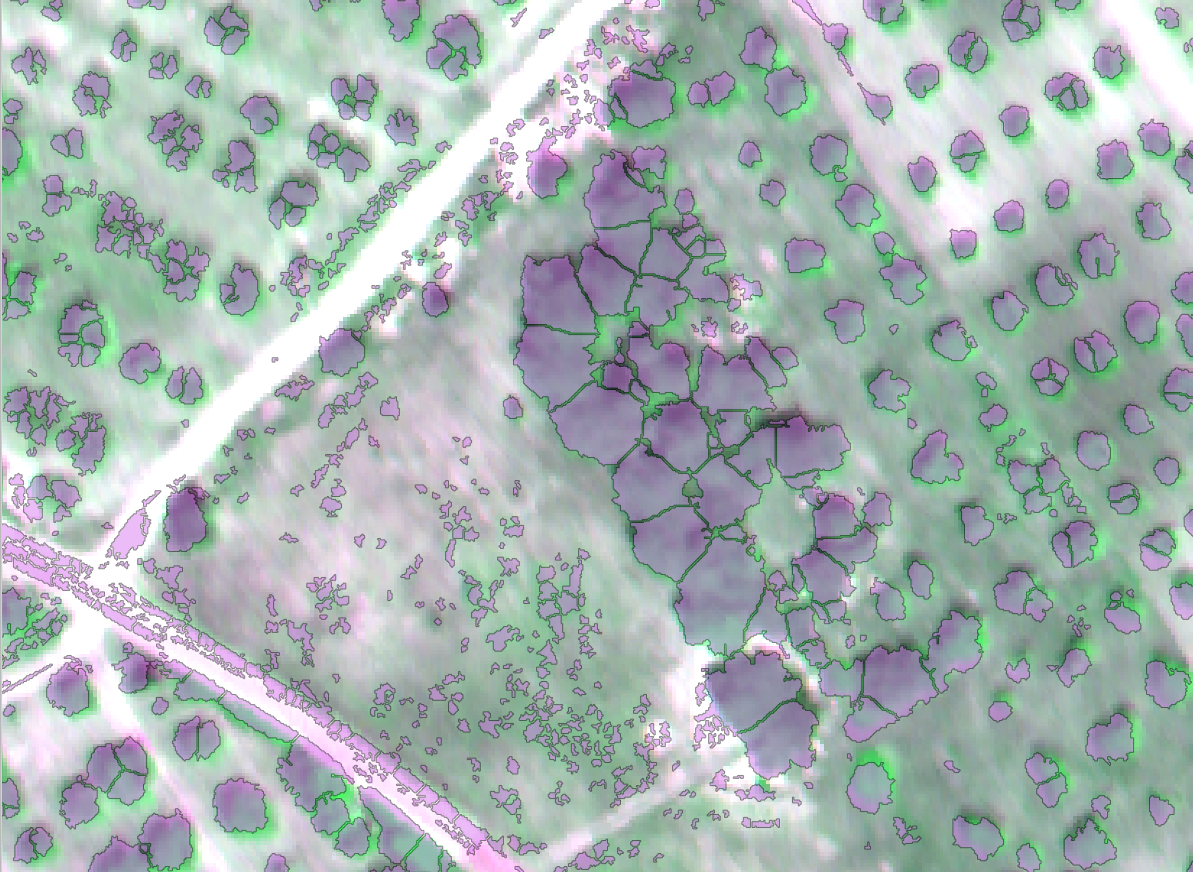
\includegraphics[height=\paperheight,width=\paperwidth]{bg_coverpage}}
\begin{frame}[plain]
\titlepage
\end{frame}}

\Large

\transdissolve<5>

\begin{frame}
  %\frametitle{Introduction}
 Resources available:
  
\begin{table}
\begin{tabular}{lclc}
 Tesla & 139.191.148.131 & /data/canhemon\\
 HPC-MPI & hpc-gw1.jrc.it & /home/hpctest\\
 HPC-EOSSSD & ? & ?\\
 \end{tabular}
\end{table}

\end{frame}

\transdissolve<5>

\begin{frame}
  \frametitle{Processing chain}
\begin{center}
\begin{itemize}
 \item Fiji/ImageJ sh => Tree crowns identification NDVI-based
 \item GRASS sh => Tree crown statistics into shp file
 \item Crown Indices sh => Additional indices from refl in shp
\end{itemize}
\end{center}
\end{frame}

\transdissolve<5>

{\usebackgroundtemplate{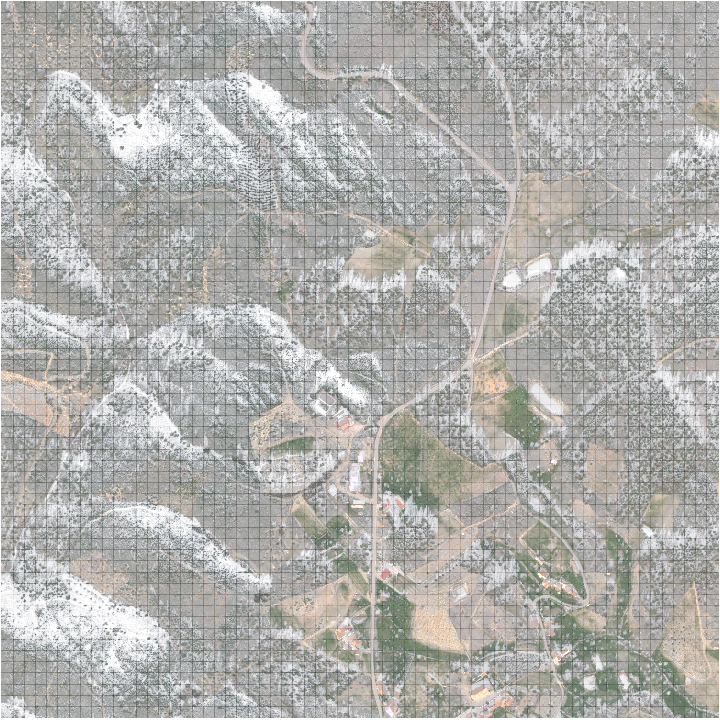
\includegraphics[height=\paperheight,width=\paperwidth]{bg_sub_64_64.png}}
\begin{frame}[plain]
\begin{shaded}
\Huge Tesla
\end{shaded}
\end{frame}}

\transdissolve<5>

\begin{frame}
  \frametitle{GRASS script}
\begin{center}
\begin{itemize}
 \item GRASS7.3 in Tesla
 \item GRASS7 => RGBNIR (Acc port)
 \item GRASS7 => thermal.sh (original port)
 \item GRASS7 => rgbnir.sh (original port)
 \item \textcolor{green}{TODO: think about RGBNIR+Hyperspectral}
\end{itemize}
\end{center}
\end{frame}

\transdissolve<5>

\begin{frame}
  \frametitle{Tree crown creation}
\begin{center}
\begin{itemize}
 \item Mask out villages from LU
  \item Processed Area 51 (future batch sample)
 \item Mask in shadow area and reprocess Tree Crown detection
\end{itemize}
\end{center}
\end{frame}

\transdissolve<5>

{\usebackgroundtemplate{\includegraphics[height=\paperheight,width=\paperwidth]{shadow.png}}
\begin{frame}[plain]
\end{frame}}

\transdissolve<5>

\begin{frame}
  \frametitle{Cal Val}
\begin{center}
\begin{itemize}
 \item Recursive v.what.rast
 \item Recommend to have a single shp file for all
 \item \textcolor{green}{TODO: QGIS PostGIS read from Andrew's}
 \item \textcolor{green}{TODO: Script to create accuracy matrix}
\end{itemize}
\end{center}
\end{frame}

\transdissolve<5>

{\usebackgroundtemplate{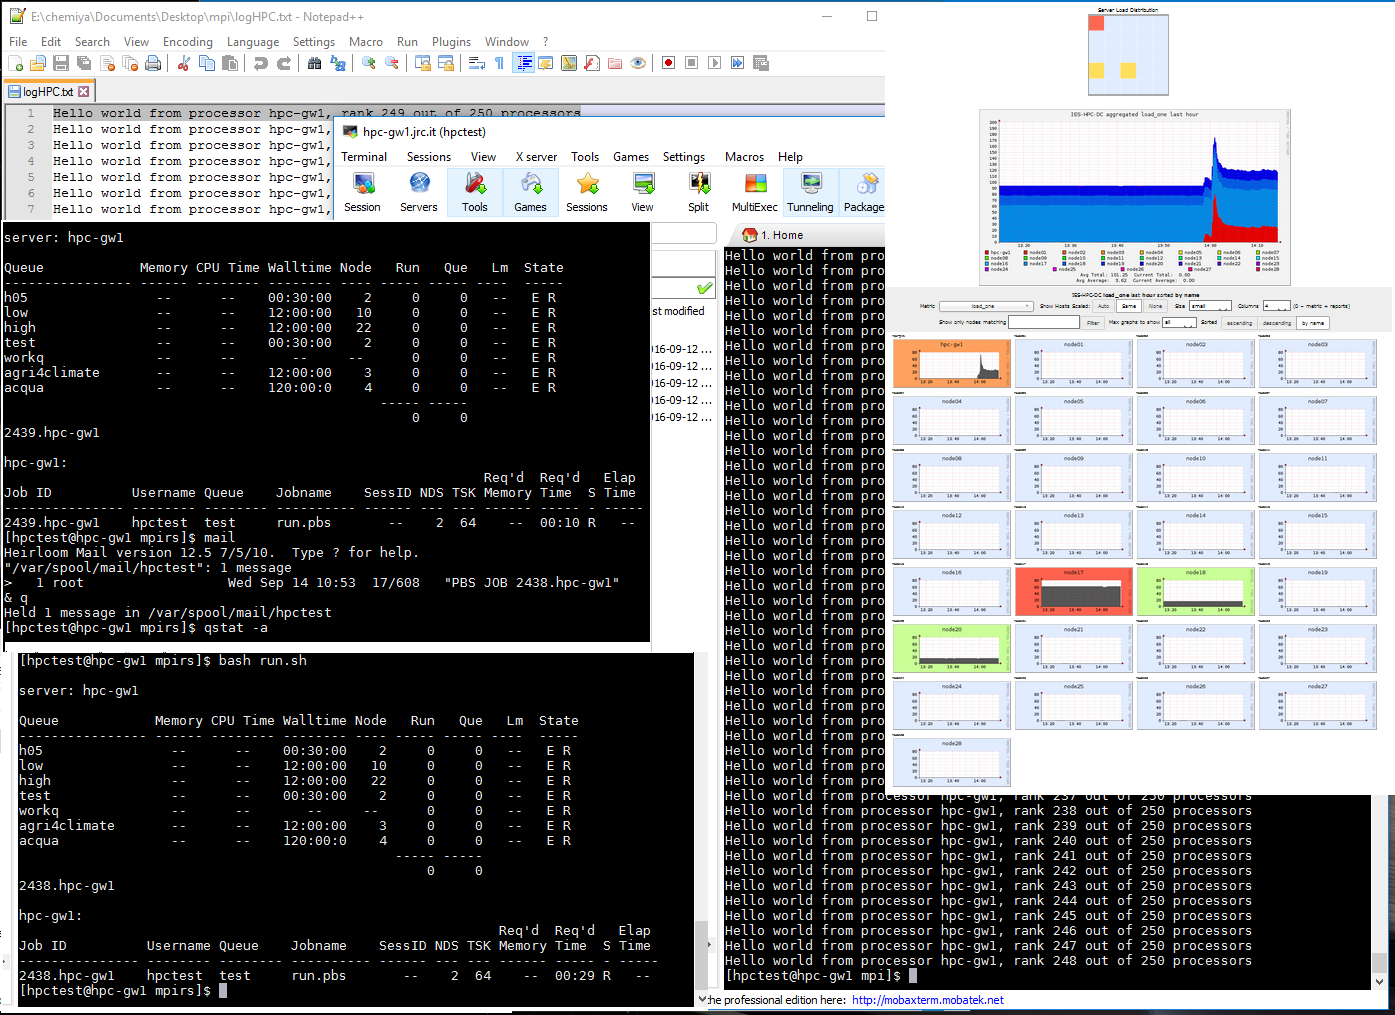
\includegraphics[height=\paperheight,width=\paperwidth]{bg_hpc_mpi.png}}
\begin{frame}[plain]
\begin{shaded}
\Huge HPC-MPI
\end{shaded}
\end{frame}}

\transdissolve<5>

\begin{frame}
\begin{center}
\begin{itemize}
 \item MPI + OpenMP hydbrid
 \item distRS test OK
 \item PBS qsub issues, libGDAL not in cores only in FE 
 \item still a test user (2 nodes, 64 cores, 30min)
 \item \textcolor{green}{Adrian trying to add libgdal module}
 \item R 3.3.1 is available on all nodes (future/different research)
\end{itemize}
\end{center}
\end{frame}

\transdissolve<5>


{\usebackgroundtemplate{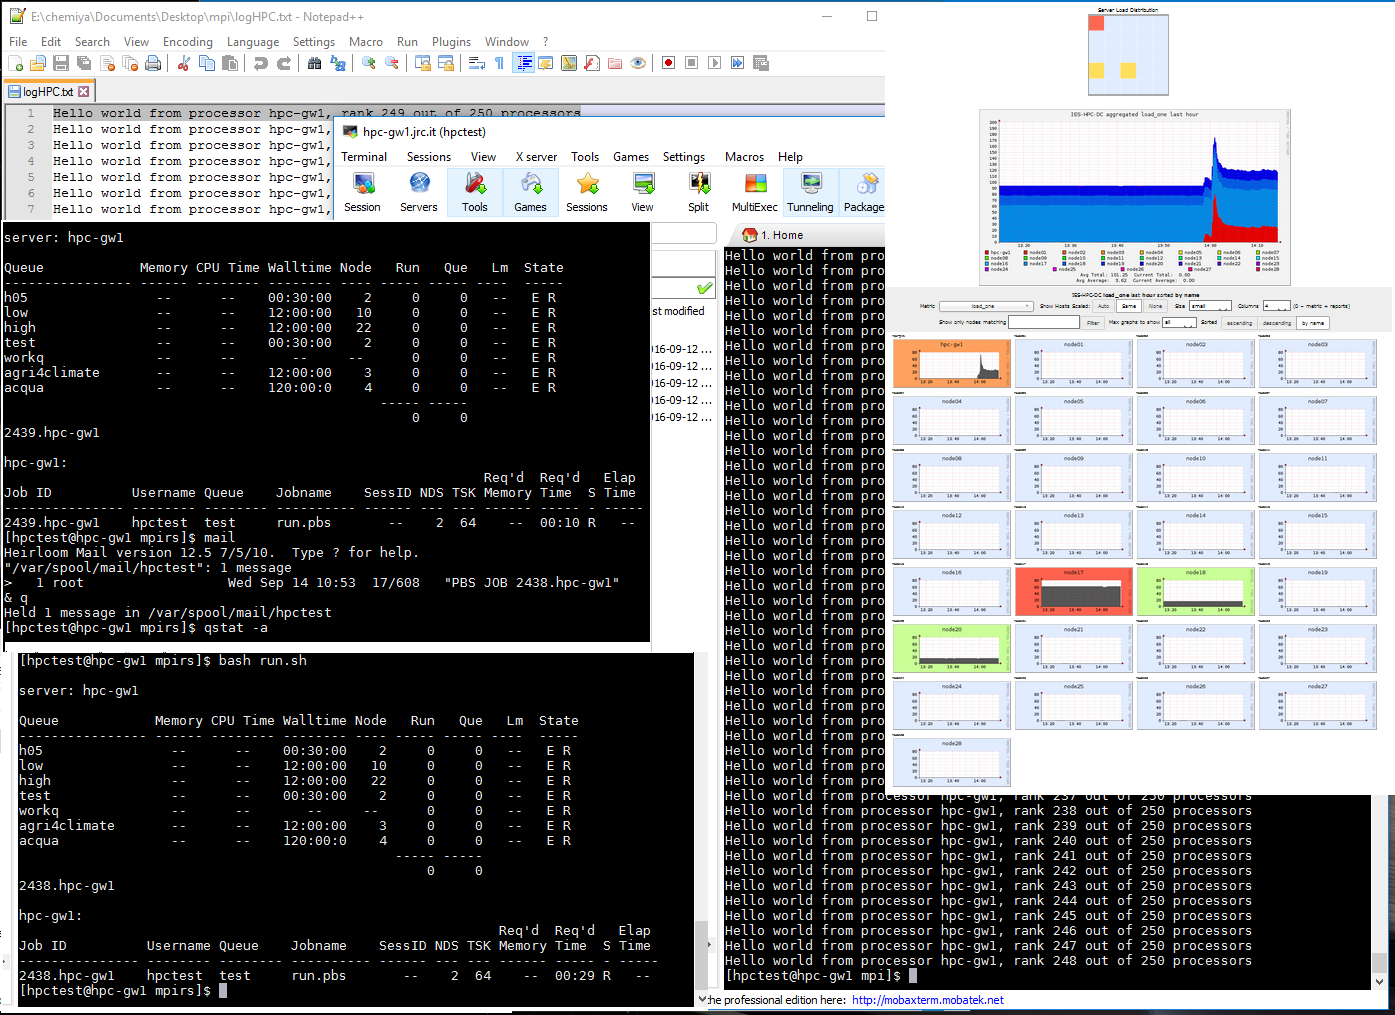
\includegraphics[height=\paperheight,width=\paperwidth]{bg_hpc_mpi.png}}
\begin{frame}[plain]
\begin{shaded}
\Huge HPC-EOSSSD
\end{shaded}
\end{frame}}

\transdissolve<5>

\begin{frame}
\begin{center}
\begin{itemize}
 \item Dockerfile
 \item Debian:testing
 \item ImageJ/Fiji \textcolor{green}{TODO: FIJI v2 !}
 \item GRASS-SVN compilation on build (v7.3)
 \item \textcolor{green}{TODO: Use the CanHeMon scripts with it}
 \item \textcolor{green}{TODO: Strategy on data distribution}
 \item \textcolor{green}{TODO: meet Dario and Pieter K (today or tomorrow)}
\end{itemize}
\end{center}
\end{frame}

\transdissolve<5>

%\begin{frame}
%  \frametitle{Water Level Virtual Gauge}
%\begin{columns}
%\column{0.45\textwidth}
%\begin{center}
%\begin{itemize}
 %\item Landsat Imagery
 %\item Water line
 %\item 12cm V. accuracy
 %\item 10-700Km2
 %\item Next: \\Orbital Altimetry 
%\end{itemize}
%\end{center}
%
%\column{0.5\textwidth}
%\begin{center}
% 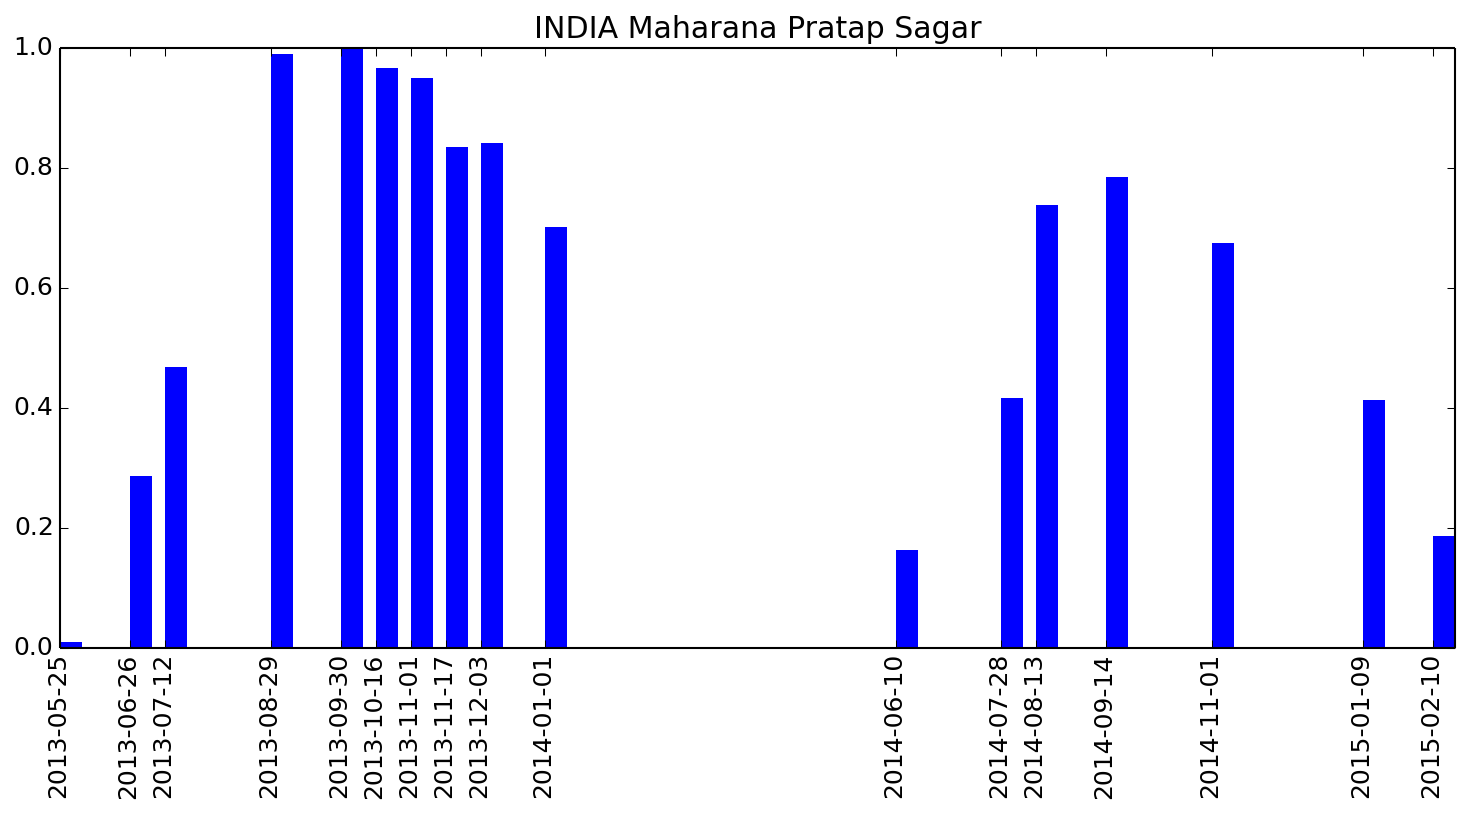
\includegraphics[height=3cm]{IN_Maharana_Pratap_Sagar_wLVG1}
% %\includegraphics[height=2.5cm]{PK_TarbelaDam_wLVG1)\\
% %\includegraphics[height=3cm]{EG_AswanDam}
%\end{center}
%\end{columns}
%\end{frame}

%\transdissolve<5>

%\begin{frame}
%  \frametitle{Equations}
%  Equations are easy
%  \begin{itemize}
%  \item Just copy and paste equations\pause
%  \item From the paper!
%    \begin{equation*}
%      \textbf{p}^* = \underset{\textbf{p}}{\arg\!\min}~\sum_{\textbf{x}}\left[ I(\textbf{W}(\textbf{x};\textbf{p})) - T(\textbf{x}) \right]^2
%    \end{equation*}
%  \end{itemize}
%\end{frame}
%
%\transdissolve<5>

%\begin{frame}
%  \frametitle{A Movie}
%  \begin{center}
%    \movie[height=5cm,width=6.5cm,poster,autostart,loop]{}{video1.avi}
%  \end{center}
%  \begin{itemize}
%  \item Movies only seem to work in Adobe Reader
%  \item Movie file is not embedded, it must be on the computer
%  \end{itemize}
%\end{frame}

\transdissolve<5>

{\usebackgroundtemplate{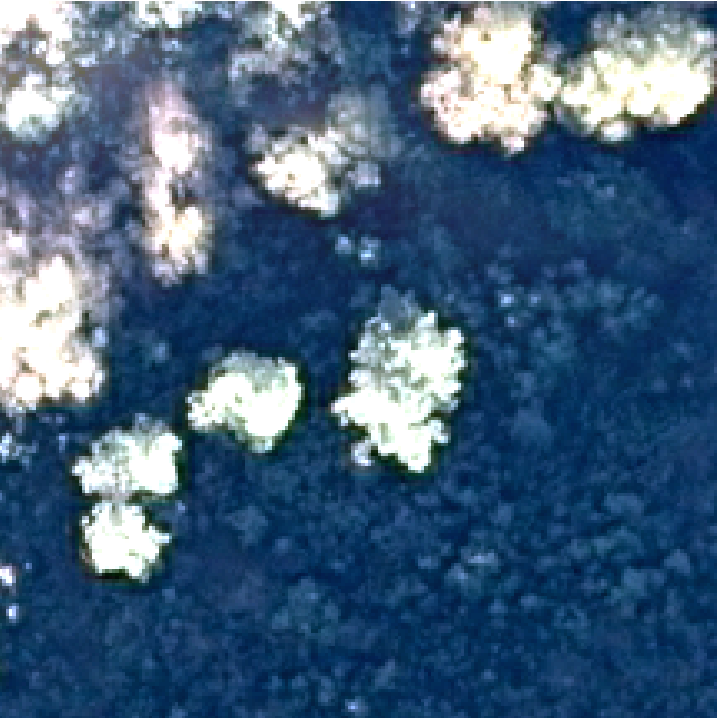
\includegraphics[height=\paperheight,width=\paperwidth]{bg_crowns.png}}
\begin{frame}[plain]
\begin{shaded}
\Huge Thank you
\end{shaded}
\end{frame}}
\end{document}
